% !TEX TS-program = xelatex
% !TEX encoding = UTF-8 Unicode
% !Mode:: "TeX:UTF-8"

\documentclass{resume}
\usepackage{zh_CN-Adobefonts_external} % Simplified Chinese Support using external fonts (./fonts/zh_CN-Adobe/)
%\usepackage{zh_CN-Adobefonts_internal} % Simplified Chinese Support using system fonts
\usepackage{linespacing_fix} % disable extra space before next section
\usepackage{cite}
\usepackage{graphicx} % import graphicx, display images
\usepackage{tabularx} % import tabularx, use tables 
\usepackage{makecell}
\usepackage{lastpage}

\usepackage{fancyhdr}	% 页脚包
%===================定义以下的样式名称为first, 表示将在标题页使用的样式===================
%\fancypagestyle{first}{	
%\fancyhf{}		%清空初始样式
%\lhead{PP 101,139101 (2022)}	%left head, 左侧页眉
%\chead{{\large\textbf{ PHYSICAL REVIEW LETTERS }}}	%center head, 中间页眉
%\rhead{\today}	%右侧页眉
%\lfoot{0031-9007/08/101(5)/057006(4)}	%左侧页脚
%\cfoot{\thepage}	%中间页脚
%\rfoot{\copyright~ 2022 The Chinese Physical Society}	%右侧页眉
%\renewcommand\headrulewidth{1pt}	%页眉线改宽度
%}
%===================定义以下的样式名称为style, 表示将在正文页使用的样式===================
\fancypagestyle{stylex}{
\fancyhf{}
\lfoot[L]{\textsc{\today}}	%左侧页脚
\cfoot{\textsc{\thepage/\pageref*{LastPage}}}	%中间页脚
\rfoot[R]{\textsc{\copyright~2024 Roy Zuoyan Shang's Résumé}}	%右侧页眉
\renewcommand{\headrulewidth}{0pt}
%\renewcommand{\footrulewidth}{1pt}
}
\pagestyle{stylex} % 应用页眉页脚定义

\title{Résumé}
\date{\today}
\author{Roy Zuoyan Shang}

\begin{document}


% arabic to use arabic numerals (default option),
% roman to use lowercase roman numerals,
% Roman to use uppercase roman numerals,
% alph to use lowercase letters and
% Alph to use uppercase letters.
% 1)gobble,不显示页码 2)arabic,阿拉伯数字页码 3)roman,罗马数字页码
%\pagenumbering{Roman} % suppress displaying page number


\begin{table}[!ht]
\flushleft
\begin{tabular}{lc}
\begin{minipage}{0.20\columnwidth}
    \flushleft
    {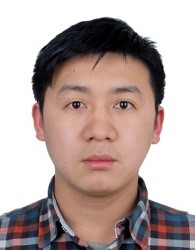
\includegraphics[width=0.8\textwidth]{./images/00.jpg}}
\end{minipage}& \begin{minipage}{.76\textwidth}\raggedright
  \pinfo{尚祚彦 | Roy(Zuoyan)Shang}{1981/01/26,Nanjing}\leavevmode\\
  \wwwinfo{(+86) 13913834668}{shangzuoyan@hotmail.com}{https://shangzuoyan.github.io}
  \end{minipage}
\end{tabular}
\end{table}

 
\section{Self-assessment}
> Proficient in \textsc{C}/\textsc{C++}/\textsc{C\#}, \textsc{Java}, \textsc{Python} and \LaTeX programming languages.										\newline
> Familiar with \textsc{TCP/IP} protocols, network programming, and proficient in design patterns.			\newline
> Familiar with \textsc{Qualcomm}/\textsc{Mediatek}/\textsc{HiSilicon} platforms.											\newline
> Familiar with Android/Tizen/FFOS systems and mainstream RTOS (FreeRTOS/RT-Thread).				\newline
> Good system architecture design ability and embedded system programming development experience.	\newline
> Good English skills, strong communication skills, and overseas work experience.				\newline
> Sincere, practical, hardworking, strong learning ability, and teamwork spirit.					\newline
> Healthy, cheerful, and responsible.															\newline
\textbf{currently working for CAIC}
\spaceline{}

\section{Education}
\edublock{2006.09-2009.06}{Cartography and Geographic Information Systems (Master of Science)}{School of Geographical Sciences,}{Nanjing Normal University (NJNU)}

\edublock{1999.09-2003.07}{Industrial Design Engineering (Bachelor of Engineering)}{School of Mechanical Engineering,}{Jiangsu University (JSU)}

\spaceline{}

\section{Skills}
\begin{itemize}[parsep=0.2ex]
  \item \textbf{Programing Language}: C, C++, C\#, Java, Python, Shell
  \item \textbf{Operating System}: Linux/Redhat, SeL4/L4Re/HelenOS, FreeRTOS/RT-Thread/Nucleus/QNX
  \item \textbf{Key words}: GDB(Gef)/Lauterbach Trace32/ARM/RSIC-V/QEMU/Gem5
\end{itemize}

% \end{itemize}
\spaceline{}

\section{Work Experience}
% E:1============================================================
\expblockex{2021.06-present}{Manager of Basic S/W Dept. / Operating System Specialist}{China Automotive Innovation Corperation,.Ltd[CAIC]}{Basic Software Dept., Intelligent Connected Business Unit}
\explistitemx{
  \begin{itemize}
    \item \textbf{Responsible for the design and development work of the operating system, including:} \\
  The design and development work of product lines such as CAIC OS / CAIC Hybrid OS / CAIC Hypervisor / CAIC Hypervisor Light, etc. \\
  The adaptation work of the NXP i.MX8QM / TI TDA4 / MTK8675 platforms. 
  \item \textbf{Some joint research and development projects: }\\
  Responsible for the system reconfiguration design, research and development, and certification work of the Siemens / Mentor Graphics Nucleus operating system cooperative project; \\
  Responsible for the system design and development work of the Zhongling Zhixing virtualization system Raite Hypervisor cooperative project; \\
  Responsible for the system design, research and development, and certification work of the lightweight virtualization system project of Renesas RH850/U2A/U2B; \\
  Responsible for the Zonal architecture AUTOSAR CP system on the lightweight virtualization solution based on the body control domain; \\
  Responsible for the system design and development work of the Horizon Robot J3/J5 assisted automatic driving operating system cooperative project.
  \end{itemize}
}
\spaceline{}

% E:2============================================================
\expblockex{2017.10-2021.01}{Specialized Manager of Wireless and Protocol Dept.}{FIH Communications(Nanjing) Co., Ltd}{Nanjing R\&D Center, IDM Business Unit}
\explistitemx{
  \begin{itemize}
    \item \textbf{Fully responsible for the system design, research and development, and certification work of Sharp (SG1/HD1/VGO/VG2) and Nokia (ROO/TAS) projects.}
  Proficient in subsystems and modules such as WLAN/Bluetooth/FM/GNSS, NFC/Felica, IR, etc., 
  participated in the research and development of the Apple ICAR Connectivity interactive scenarios 
  participated in the joint research and development work of Byton smart cockpit.
    \item \textbf{Some outsourced businesses:}
  Fully responsible for the design, research and development, and certification work of the wireless communication related subsystems of the Vivo Khronos project;
  Fully responsible for the design, research and development work of the wireless communication related subsystems of the Mi D1S OTA project;
  Fully responsible for the design, research and development, and certification work of the wireless communication related subsystems of the Mi J15s project;
  Fully responsible for the design, research and development, and certification work of the wireless communication related subsystems of the LG DH0 project.
  \end{itemize}
}
\spaceline{}

% E:3============================================================
\expblockex{2016.01-2017.10}{S/W Specialist->Director of Terminal OS Dept.}{Jiangsu HopeRun Software Co., Ltd}{Terminal OS Dept., Intelligent Terminal Business Unit}
\explistitemx{
  \begin{itemize}
    \item \textbf{Take over the AtelierOS project of Euler Laboratory in Huawei Central Software Institute:}
  AtelierOS is a virtual container based on the L4 microkernel, on which multiple operating systems can be deployed and run and perform seamless switching.
  Responsible for the overall system architecture design and implementation, and adapt to the evolution of Huawei Mate series.
    \item \textbf{Take over the Texas AT&T project of Huawei Terminal Company:}
  Based on the Qualcomm MSM8939 platform, as the project technical leader, responsible for system Bringup, certification work, and problem tracking.
    \item \textbf{Take over the VR project of Huawei Terminal Company:}
  Responsible for the system architecture and design of the project, and responsible for the development and coding work of key subsystems.\\
  Based on the restructured gSOAP OnVIF service, the inter-process communication service based on libevent, and the DAL encapsulation based on SQLite.
    \item \textbf{ Take over the Smart Watch Turnkey project of ClouderSemi Company:}
  Responsible for the system architecture and design of the project, and responsible for the development and coding work of the system framework based on Bluetooth.
  Based on the private protocol of signaling interaction of Bluetooth LE, the transmission service based on Bluetooth RF-COMM, and the audio service of Bluetooth HFP/A2DP.
  \end{itemize}
}
\spaceline{}

% E:4============================================================
\expblockex{2013.05-2016.01}{Principal S/W Engineer->Manager of Wireless Dept.}{Yulong Computer Telecommunication Scientific(Shenzhen) Co., Ltd}{The 52rd Dept., Nanjing R\&D Center}
\expitemx{
  Coolpad overseas market product R \& D; 
  mainly responsible for the Bringup of Connectivity related modules WLAN / BT / FM Combo (Integrated) WCN3660 / WCN3620 / WCN3620B / WCN3610 chips, related module maintenance, control of certification tests (WFA / BQB, BT-IOT, etc.), communication of related requirements of overseas operators, and rapid resolution of overseas online testing problems. [GNSS] Configuration of WTR1605L / WTR4905 Transceiver, SKY65611-11 PA (eLNA) chips (this work is included in the RF Bringup work), to solve problems in AGPS testing and SUPL1.1 / 2.0 certification testing; [NFC] Bringup of NXP PN544 / PN547 chips, driver debugging, NFC protocol stack upgrade, SmartCard solution integration, EMVCo2.3.3 certification, and support for VISA / MASTERCARD / AMEX payment functions; [IR] Bringup of ABOV MC96FR116CU chips, and driver debugging work; completed the development work of new requirements of TMO operators, including DeviceReporting, HW Encyption, Anti-theft Feature, etc. 
  Related platforms involved are as follows: MSM8926 (Vodafone Smart 4 Max) / MSM8916 (Panasonic ELUGA L 4G) / MSM8909 (China Mobile Y75) / MSM8939 (Qikoo), etc.
}
\spaceline{}

% E:5============================================================
\expblock{2009.10-2013.05}{Sr. S/W Engineer->Manager of S/W Dept.}{TeleEpoch Co., Ltd}{Software Dept., Nanjing R\&D Center}
\expitemx{
  [Qualcomm AMSS8960 platform] G6611/G3617 project / [Qualcomm AMSS8625 platform] QRD-G2616/G3616/G3617 project:\\
  Mainly responsible for the modem side software, and undertake the implementation of the telephony-related code in the Android Framework/RIL and QCRIL layers.
  [Qualcomm AMSS7627 platform] F3610/F3611 project:\\
  Mainly responsible for the modem side software, responsible for the related code implementation in the Android Framework/RIL and QCRIL layers, and responsible for the IOT Level2 test (in the US Foveros Nokia network laboratory).
  [Qualcomm QSC6085 platform] CDMA 1x EVDO M600 project:\\
  (Resided in the US for 1 year) Mainly responsible for the MMS, WAP browser, and WWW (Full HTML) browser modules, and was responsible for the MMS/WAP IOT test (in the US Foveros Motorola network laboratory), and discussed functional requirements and technical support matters with PCD, UMX, and US Cellular. Based on the Qualcomm QSC6085 platform.
  [Qualcomm QSC6055 platform] CDMA 1x WMDP project:\\
  Mainly responsible for the application modules of automatic speech recognition [ASR] (iFlyTek of University of Science and Technology/VoiceSignal Tech), and gravity sensor [G-Sensor]. Exhibited at CES2010 and the Asia Telecom Exhibition.
  [Qualcomm QSC6270 platform] GSM/WCDMA WA01/WA02/WA02 (DSDS)/W399/W599/W599 (DSDS)/E7610/E7620 project:\\
  Undertake the underlying driver work, including: FLASH driver (Micron/Hynix), LCD/MDP driver (Sunrise of Songrui/Truly, etc., LCM driver IC includes TM2.0 3.55 ILI9341 9225 9225G HX8340B 8347D), T9 keyboard/QWERTY keyboard driver, and the debugging of the HALL device flip device driver, and the underlying implementation work of GSDI dual-card support; undertake the work of the OEM interface encapsulation layer and the application layer; be responsible for the modules such as SMS (GSM 03.38/03.40/07.05), MMS (TS23.140/OMA), STK (GSM 11.14), SIM card (TS 31.102), Bluetooth, Brew JavaVM, WWW (Full HTML) browser, multimedia, and input method.
  [Qualcomm MDM6085 platform] CDMA 1x EVDO D2/D3/D5 data card project: \\
  Mainly responsible for the development and debugging tasks of the lower computer AT commands and the upper computer synchronization and dialing software.
}
\spaceline{}

% E:6============================================================
\expblockex{2006.07-2009.05}{Graduated Student}{National Key Laboratory of Virtual Geographic Environment[VGEKL]}{Ministry of Education + Nanjing Normal University (NJNU)}
\expitemx{
  [2007.11-2009.05] Research on the key technologies of 3D GIS for underground space entities based on the non-manifold theory\\
Project Number: 2007AA12Z236 [National 863 Project]\\
Engaged in the research of 3D GIS framework construction (OSGi RCP framework), spatial data indexing (the algorithm implementation and application of general search tree GiST, space index library Space Index Library, and hybrid index OR-tree), and data visualization (Open Inventor, IRRLicht, OSG, Coin3D), and was responsible for the development task of the prototype system.\\
  [2006.10-2007.03] Research on the key technologies for the copyright protection of GIS vector data products\\ 
Project Number: 2006AA12Z222 [National 863 Project]\\
Engaged in the research of pseudo-random sequence key masks (maximum length linear shift register m-sequence, M-sequence, Golden sequence, and chaotic sequence), watermark embedding and extraction, wavelet decomposition and reconstruction, and performed watermark embedding on high-dimensional spatial data to achieve the purpose of protecting spatial data, and participated in the completion of the development task of the prototype system.\\
}
\spaceline{}

% E:7============================================================
\expblock{2003.10-2006.08}{S/W Engineer}{AMOI Electronics Co., Ltd}{Communication Dept., Nanjing Research Institute}
\explistitemx{
  \begin{itemize}
    \item \textbf{Related platforms and operating systems:}\\
    Spreadtrum platform, X-Thread RTOS.\\
    Qualcomm platform, Rex OS/Brew/BrewMP system.\\
    Toshiba platform, iTRON system.
    \item \textbf{Responsibilities in the project:}\\
  Mainly responsible for the software development tasks of the PHS and Smartphone.\\
  MMI driver, LCD driver, and functional business modules (PIM card PIN module, phonebook module, and schedule module) application programs.\\
  Accumulated rich project development experience, became familiar with the protocols and file structure of PIM, and had an in-depth understanding of the iTRON system. \\
  And served as the software group leader in the S368 project. 
  \end{itemize}
  % Responsible for the overall planning of the software development tasks of the entire project and software version control.\\
}
\spaceline{}

%\hspace*{4em}\parbox[c]{\textwidth-4em}{ }


% ============================================================
\section{Publications and Commitments}
% increase linespacing [parsep=0.5ex]

\textsc{Co-author of 3 publications}

[1] Xu H, Lu G, Sheng Y, Guo F, \textbf{Shang Z}.3D GIS spatial operation based on extended Euler operators[J].\newline
  Proceedings of SPIE - The International Society for Optical Engineering, 2008, 7143:71433D-71433D-10.\newline
  DOI:10.1117/12.812655.\newline
[2]\textbf{尚祚彦}.3D GIS混合空间索引技术研究[D].南京师范大学,2009.DOI:10.7666/d.d183065.\newline
[3]张璐,柴燕妮,王丹,\textbf{尚祚彦}.基于地理国情的县域生态环境质量评价研究[J].地理空间信息, 2022, 20(10):79-81.

\textsc{Co-inventor of 5 patents}

\begin{tabularx}{\textwidth}{|p{7.2em}|X|p{6.8em}|}
\hline
\makecell[lt]{Patent Number} & \makecell[lt]{Patent Description} & \makecell[lt]{Publication Date}\\
\hline
[CN115480934A] & 专利一种分布式数据处理的方法、装置、设备及储存介质 & 2022/12/16\\
\hline
[CN114153560A] & 专利一种虚拟中断处理方法、装置、设备及介质 & 2022/03/08\\
\hline
[CN114579556A] & 专利一种数据处理方法、装置、设备及存储介质 & 2022/06/03\\
\hline
[CN114579556B] & 专利一种数据处理方法、装置、设备及存储介质 & 2022/08/02\\
\hline
[CN114298990A] & 专利一种车载摄像装置的检测方法、装置、存储介质及车辆 & 2022/04/08\\
\hline
[CN114500408A] & 专利一种以太网络交换装置、数据处理装置和车辆 & 2022/05/13\\
\hline
\end{tabularx}




  
  


%% Reference
%\newpage
%\bibliographystyle{IEEETran}
%\bibliography{mycite}
\end{document}
